%% Los cap'itulos inician con \chapter{T'itulo}, estos aparecen numerados y
%% se incluyen en el 'indice general.
%%
%% Recuerda que aqu'i ya puedes escribir acentos como: 'a, 'e, 'i, etc.
%% La letra n con tilde es: 'n.

\chapter{Métodos}
%\setcounter{section}{1}
\section{Métodos estadísticos}

Este capítulo tiene como objetivo focalizar al lector en los aspectos fundamentales sobre los que se apoya este trabajo. Se compone de tres secciones, en la primera se presenta la metodología estadística que se incluirá en el paquete de R.  En la segunda y tercera sección, se presenta un flujo de trabajo reproducible para el desarrollo del paquete y la aplicación web Shiny, respectivamente.



\subsection{Modelo AMMI y SREG}
El modelo AMMI (Zobel et al. 1988) y SREG (Cornelius et al. 1996; Crossa y Cornelius 1997 y 2002) son modelos multiplicativos que además de tener una componente  aditiva, poseen una multiplicativa. Ellos difieren en las componentes aditivas que se eliminan de la ecuación y que se incorporan en forma multiplicativa. Mientras que AMMI considera los ambientes (A) y el genotipo (G) como aditivos, SREG solo A. Por lo tanto, en el primero la IGA representa la parte multiplicativa y en el segundo G e IGA en forma conjunta. 

Los parámetros multiplicativos, tanto en el modelo AMMI como en el SREG, se estiman por medio de la Descomposición en Valores Singulares (DVS) de la matriz que contiene los residuos para cada combianción de genotipo y ambiente luego de ajustar por mínimos cuadrados el modelo de efectos principales. 

Las ecuaciones de los distintos modelos son:

\hspace{0.5cm} AMMI: $y_{ij}= \mu + G_i + A_j + \sum_{k=1}^K \lambda_k \alpha_{ik} \gamma_{jk}$

\hspace{0.5cm} SREG: $y_{ij}= \mu + A_j + \sum_{k=1}^K \lambda_k \alpha_{ik} \gamma_{jk}$ 

donde 
\begin{itemize}
\item $y_{ij}$ es el caracter fenotípico evaluado (rendimiento o cualquier otro caracter de interes) del $i$-ésimo genotipo en el $j$-ésimo ambiente,
\item $\mu$ es la media general,
\item  $G_i$ es el efecto del $i$-ésimo genotipo con $i=1,...,g$,
\item $A_j$ es el efecto del $j$-ésimo ambiente con $j=1,...,a$,
\item $\sum_{k=1}^K \lambda_k \alpha_{ik} \gamma_{jk}$ es la sumatoria de términos multiplicativas utilizadas para modelar la IGA en AMMI o G e IGA en SREG. Siendo, K el número de términos multiplicativos retenidos en el modelo con $K \leq min(g-1,a-1)$ en AMMI y $K \leq min(g,a-1)$ en SREG; $\lambda_k$ el $k$-ésimo valor singular y $\alpha_{ik}$ y $\gamma_{jk}$ el elemento del autovector asociado con el $i$-ésimo genotipo y el $j$-ésimo ambiente para el $k$-ésimo término multiplicativo. Generalmente los dos primeros términos multiplicativos ($K=2$) son suficientes para explicar los patrones de la IGA en AMMI y de G e IGA en SREG; la variabilidad remanente se interpreta como ruido aleatorio. 
\end{itemize}


El resultado de los dos primeros términos multiplicativos de la SVD se presenta a menudo en un biplot llamado GE (\emph{Genotipe-Environment}) (\textbf{CITA}) en AMMI y GGE en SREG (Yan et al. 2000) y representan una aproximación de dos rangos de los efectos multiplicativos. Dado que para seleccionar cultivares, el efecto de G e IGA debe considerarse simultáneamente, el modelo SREG resulta superior a AMMI para visualizar patrones en datos EMA. Un biplot GGE que explica suficiente variabilidad debida a G e IGA de un conjunto de datos MET permite, entre otras cosas, la visualización de tres aspectos importantes: 

\begin{itemize}
\item[(i)] las relaciones entre los genotipos y ambientes representadas por el patrón \emph{which-won-where}, que facilitan la investigación del megaambiente (Gauch y Zobel, 1997);

\item[(ii)] las interrelaciones entre los ambientes de prueba que permiten la identificación de mejores para la evaluación de cultivares (Cooper et al., 1997) y de aquellos redundantes que pueden ser descartados (Yan y Rajcan, 2002);

\item[(iii)] las interrelaciones entre genotipos que posibilita la comparación entre ellos y la clasificación de los mismos considerando tanto en el rendimiento medio como la estabilidad (Yan et al., 2001)
\end{itemize}

En un biplot, el i-ésimo genotipo se muestra como un punto definido por todos los valores $g_{ik} = \lambda_k^{s} \gamma_{ik}$, y el j-ésimo ambiente por $e_{kj} = \lambda_k^{1-s} \delta_{jk}$ ($k=1,2$ para un biplot bidimensional), donde $s$ es el factor de partición. Cuando $s=1$ se denomina escalamiento centrado en los genotipos, centrado en los ambientes si $s=0$ y simétrica cuando $s=0.5$. El último factor es el utilizado en el biplot GE y el más utilizado en GGE, aunque dependiendo de los intereses de la investigación, se pueden construir numerosos biplots derivados de SREG. Independientemente del factor de partición utilizado, los biplots GGE revelan el mismo patrón \emph{which-won-where}. Sin embargo, difieren en diversos aspectos. El primero muestra la interrelación entre genotipos con mayor precisión que cualquier otro método, el centrado en el ambiente es el más informativo de las interrelaciones entre los ambientes, mientras que el simétrico permite visualizar la magnitud relativa tanto de la variación de los genotipos como de los ambientes. 



\subsection{Modelo AMMI robusto}

El modelo AMMI, en su forma estándar, asume que no hay valores atípicos en el conjunto de datos. Sin embargo, la presencia de \emph{outliers} es más una regla que una excepción cuando se consideran datos agronómicos debido características inherentes a los genotipos que se evalúan, errores de medición o el efecto inesperado de plagas o enfermedades que pueden afecta el rendimiento de algunos genotipos.

Rodrigues et al. (2015) proponen una generalización robusta del modelo AMMI, que resulta de ajustar la regresión robusta basada en el estimador M-Huber (Huber, 1981) y luego utilizar un procedimiento DVS / PCA robusto. Consideraron varios métodos de DVS / ACP dando lugar a un total de cinco modelos robustos llamados: R-AMMI, H-AMMI, G-AMMI, L-AMMI, PP-AMMI. 

El empleo de la versión robusta del modelo AMMI puede ser extremadamente útil debido a que una mala representación de genotipos y ambientes puede resultar en un mala decisión con respecto a qué genotipos seleccionar para un conjunto dado de ambientes (Gauch1997, Yan et al. 2000). A su vez, la elección de los genotipos incorrectos pueden provocar grandes pérdidas en términos de rendimiento. Los biplots obtenidos de los modelos robustos mantienen las características e interpretación estándar del modelo AMMI clásico (Rodrigues et al., 2015).


\subsection{Métodos de imputación}


Una limitación importante que presentan los modelos multiplicativos descriptos previamente es que requieren que el fenotipo de todas las combinaciones de genotipos y ambientes se encuentre registrado, es decir no admiten valores perdidos. Aunque los EMA están diseñados para que todos los genotipos se evalúen en todos los ambientes, la presencia de valores faltantes es muy común debido a errores de medición o pérdidas de plantas por animales, inundaciones o problemas durante la cosecha, además de la dinámica propia de la evaluaciones en las que se incorporan y se descartan genotipos debido a su pobre desempeño (Hill y Rosemberg, 1985).

Se han propuesto numerosas metodologías para superar el problema de valores ausentes en el conjunto de datos, entre las cuales se encuentran:

\begin{itemize}
\item EM-AMMI: Gauch y Zobel (1990) desarrollaron un procedimiento iterativo que utiliza el algoritmo de maximización de la esperanza (EM, del inglés \emph{Expectation-Maximization}) incorporando el modelo AMMI. 
\end{itemize}
\begin{itemize}
\item EM-SVD: Perry (2009) propone un método de imputación que combina el algoritmo EM con DVS. 
\end{itemize}
\begin{itemize}
\item EM-PCA: Josse y Husson (2013) proponen imputar los valores faltantes de un conjunto de datos mediante un ACP.
\end{itemize}
\begin{itemize}
\item Gabriel Eigen: Arciniegas-Alarcón et al. (2010) presentan un método de imputación que combina regresión y aproximación de rango inferior usando DVS. 
\end{itemize}
\begin{itemize}
\item WGabriel Eigen: Arciniegas-Alarcón et al. (2014) plantean una extensión ponderada del método Gabriel Eigen.
\end{itemize}




\section{Paquete de R}

%https://oscarperpinan.github.io/R/Paquetes.html 


Un paquete de R consisten en conjuntos de funciones desarrolladas con fines específicos que se distribuyen con un protocolo determinado, garantizando su correcto funcionamiento.  Para la creación del mismo se deben seguir ciertas convenciones, existiendo elementos obligatorios y otros opcionales. Entre los primeros se encuentran:

\begin{itemize}
	\item Archivo DESCRIPTION: describe el contenido del paquete y establece cómo se va a relacionar con otros.
\end{itemize}

\begin{itemize}
	\item Carpeta R: contiene el o los archivos de código de R con las funciones del paquete.
\end{itemize}

\begin{itemize}
	\item Carpeta man: incluye archivos con la documentación del paquete, funciones y datasets.
\end{itemize}

\begin{itemize}
	\item Archivo NAMESPACE: declara las funciones del paquete que se ponen a disposición de los usuarios y de qué funciones de otros paquetes hace uso.
\end{itemize}


Los elementos opcionales que se pueden agregar son por ejemplo:

\begin{itemize}
	\item Carpeta data: contiene objetos de R que contienen datos.
\end{itemize}

\begin{itemize}
	\item Carpeta vignettes: contiene los tutoriales que muestran ejemplos de uso del paquete, generalmente escritos en Rmarkdown.
\end{itemize}

\begin{itemize}
	\item Carpeta tests: incluye código que permiten someter al paquete a diversos controles.
\end{itemize}

Para la creación del paquete, se deben instalar y cargar en la sesión de trabajo los paquetes:
 \emph{devtools}, \emph{usethis}, \emph{roxygen2}, \emph{ustestthat}, \emph{knitr}, \emph{available}. Además, en caso de utilizar el Windows se debe descargar e instalar Rtools .


\subsection{Creación del paquete}

En primer lugar se debe elegir el nombre del paquete, el cual debe cumplir con ciertas reglas: solo puede contener letras, números o puntos; tener al menos dos caracteres y empezar con una letra y no terminar con un punto. Una vez elegido el nombre, se debe chequear si el mismo está disponible en los repositorios \emph{GitHub}, \emph{CRAN} y \emph{Bioconductor}, donde se alojan los paquetes. Para ello, se utiliza el paquete \emph{available}, que además indicará si el nombre elegido tiene algún significado especial que podemos desconocer (revisa las webs de Wikipedia, Wiktionary y Urban Dictionary) (Figura \ref{fig:fig31}). 

\begin{lstlisting}
	# Cargar la libreria devtools
	library(available)
	# Crear el paquete geneticae
	available(``geneticae")
\end{lstlisting}


 \begin{figure}[H]
\begin{center}
	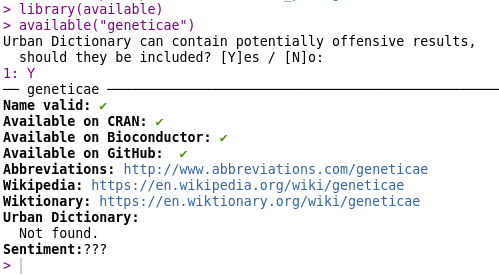
\includegraphics[width=9.5cm]{./Graficos/available.png}	
\end{center}
	\caption{Chequeo de disponibilidad del nombre elegido}
\label{fig:fig31}
\end{figure}


Para la creación del paquete se utilizán  \emph{devtools} y  \emph{usethis} que incluyen funciones que simplifican la tarea. La función \textcolor{blue}{create\_package}("nombre\_paquete") generará una carpeta con el nombre provisto (Figura \ref{fig:fig32}). Si nose especifica una ubicación entonces se creará en el directorio actual.


\begin{lstlisting}
# Cargar la libreria devtools
library(devtools)
# Crear el paquete geneticae
create_package(``/home/julia-fedora/Escritorio/geneticae")
\end{lstlisting}


 \begin{figure}[H]
	\begin{center}
		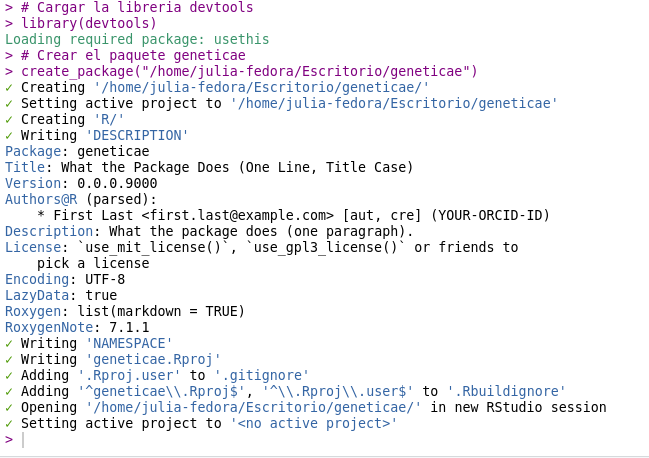
\includegraphics[width=13cm]{./Graficos/creacion.png}	
	\end{center}
	\caption{Creación del paquete geneticae}
	\label{fig:fig32}
\end{figure}


\subsection{Archivos de código}

Una vez creada la estructura del paquete se deben programar las funciones que el mismo contendrá. Cada una de ellas debe ser guardada en un archivo de extensión .R, en el subdirectorio R/. Para ello, se utiliza la función \textcolor{blue}{use\_r}() la cual crea un script ubicado en la carpeta R/, donde el código de interés será agregado. 

A medida que se va desarrollando el paquete, con funciones internas y otras que se exportan, con algunas que se relacionan entre si y que a su vez dependen de otros paquetes, se deben ir realizando pruebas para asegurarse que los creados códigos realizan lo que realmente se desea. Para ello, la función \textcolor{blue}{load\_all}() simula el proceso de construcción, instalación y carga del paquete, permitiendo probar la función de manera interactiva.

Muy frecuentemente se utilizan funciones que se encuentran disponibles en otros paquetes. La función \textcolor{blue}{use\_package}() agrega el paquete de interés a la sección Imports del archivo DESCRIPTION, y luego para llamar a las mismas dentro de una función se debe utilizar @importFrom paquete función. Alternativamente, si se utilizan repetidamente muchas funciones de otro paquete, es posible importarlas todas utilizando @import paquete. Sin embargo, esta es la solución menos recomendada porque hace que el código sea más difícil de leer, y si tiene muchos paquetes, aumenta la posibilidad de que entren en conflicto nombres de funciones.


\subsection{Documentación}

Uno de los aspectos más importantes del paquete es la documentación donde se describe cómo se usa cada función, para qué sirven los argumentos, aclarar qué tipo de resultado devuelve, proveer ejemplos para el uso, etc. El paquete \emph{roxygen2}, provee pautas para escribir comentarios con un formato especial que incluyan toda la información requerida justo antes de la definición de la función. El código y la documentación son adyacentes, de modo que cuando el código se modifique le exigirá que actualice la documentación. 

El flujo de trabajo para crear la documentación con el paquete \emph{roxygen2} es el siguiente:

\begin{itemize}
\item Agregar comentarios a los archivos .R. Estos deben comenzar con \#', para distinguirlo de los comentarios regulares, y preceden a una función. La primera oración se convierte en el título y el segundo párrafo es una descripción de la función. Para el resto de los campos de la documentación, se utilizan de etiquetas que comienzan con @, siendo las más importantes a incluir:

\begin{itemize}
\item @param: se detalla para qué sirve cada parámetro de la función.
\item @return: para explicar qué objeto devuelve la función.
\item @details: agregar cualquier aclaración que se considere necesaria.
\item @examples: incluir ejemplos de uso de la función.
\item @export: indicar que esta función tiene que estar disponible cuando alguien cargue el paquete con library(). No es necesario exportar funciones auxiliares de utilidad interna.
\end{itemize}

\item Ejecutar devtools::document() para convertir los comentarios de roxygen en archivos .Rd que compondrán el manual y que deben ir guardados en la carpeta man.
\end{itemize}


\emph{Roxygen2} permite utilizar la descripción de los parámetros de otras funciones usando @inheritParams. Esta documentará los parámetros que no están documentados en la función actual, pero que si lo están en la función fuente. La fuente puede ser una función en el paquete actual, vía @inheritParams function, u otro paquete, vía @inheritParams package::function. Además \emph{Roxygen2} permite incluir referencias utilizando @references. En caso de importar paquetes, como se indicó en la sección anterior, se deben declarar usando @importFrom o @import, previo a la definición de la función.


\subsection{Editar el archivo DESCRIPTION}

El archivo DESCRIPTION provee toda la metadata sobre el paquete que se esta creando. En este archivo hay algunos campos que tienen que estar presentes de forma obligatoria y otros que son opcionales. Los elementos obligatorios son:

\begin{itemize}
\item Package: nombre del paquete
\item Title: título del paquete (hasta 65 caracteres, Escrito De Esta Forma).
\item Version: número de la versión actual del paquete (por ejemplo, 0.2.1)
\item Author, Maintainer o Authors@R: quiénes han participado en el paquete.
\item Description: un párrafo que describa el paquete.
\item License: nombre de la licencia bajo la cual se distribuye el paquete. Si se pretende que cualquiera lo puede usar, entonces se debe recurrir a los tipos mas comunes de licencia para código abierto: CC0, MIT o GPL. Como se muestra en la Figura \ref{fig:fig33}, el paquete geneticae se encuentra bajo la licencia GPL-3. Para esto, se utilizó la función \textcolor{blue}{use\_gpl3\_license}() del paquete usethis, la cual agrega la información al archivo DESCRIPTION y además crea un archivo LICENSE al directorio del paquete.
\end{itemize}




En cambio, los elementos no obligatorios:
\begin{itemize}
\item Date: fecha de publicación de esta versión del paquete.
\item Imports, Depends, Suggests: es muy común que las funciones desarrolladas necesiten hacer uso de algunas que pertenecen a otros paquetes. Estos serán indicados en los campos Imports, Depends, Suggests del archivo DESCRIPTION. Como se muestra en la Figura \ref{fig:fig33}, en el campo Imports se indica que geneticae necesita los paquetes: stats, GGEBiplots, ggforce, ggplot2, etc. Mientras que los listados en Suggest indica que se podría hacer uso de los mismos, aunque no son indispensables. Por último, el paquete geneticae se puede utilizar en versiones de R iguales o superiores a la 2.12, como se establece en Depends.
\item URL: dirección de la página web del paquete.
\item BugReports: dirección donde los usuarios pueden enviar avisos con los problemas que encuentren al utilizar el paquete.
\end{itemize}

El archivo DESCRIPTION del paquete geneticae se muestra en la Figura \ref{fig:fig33}

 \begin{figure}[H]
	\begin{center}
		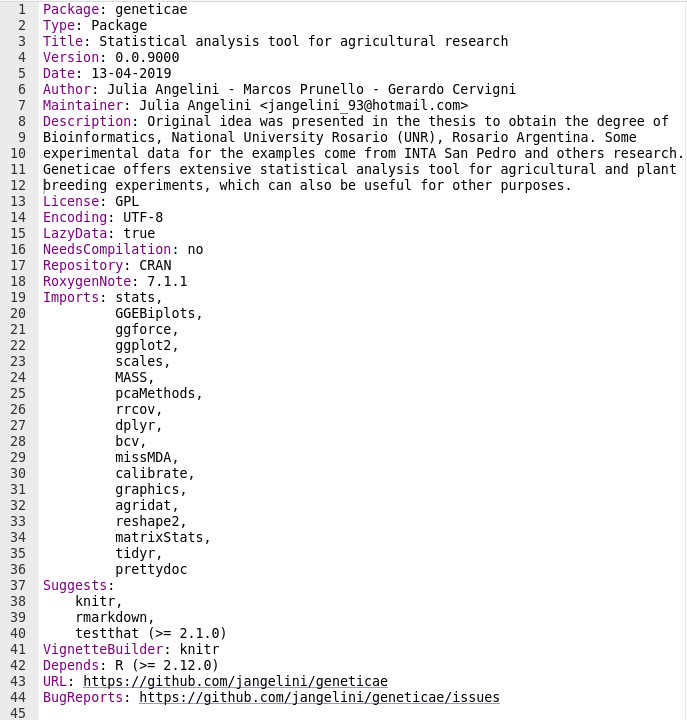
\includegraphics[width=13cm]{./Graficos/DESCRIPTION.png}	
	\end{center}
	\caption{Archivo DESCRIPTION de geneticae}
	\label{fig:fig33}
\end{figure}


\subsection{Testeos}

Las pruebas resultan fundamentales en el desarrollo de paquetes, asegura que el código haga lo que realmente se desea. Existen pruebas informales como aquellas realizadas con la función \textcolor{blue}{load\_all}() que permite que las funciones creadas estén disponible rápidamente para uso interactivo. Sin embargo, las pruebas interactivas pueden convertirse en scripts reproducibles, los cuales resultan superiores debido a que se indica explícitamente cómo debería comportarse el código, provocando que los errores solucionados no vuelvan a ocurrir. Para ello, se utiliza la función \textcolor{blue}{use\_testthat}() del paquete \emph{testthat} (Wickham,2011). Esta agrega testthat al campo Suggests en el archivo DESCRIPTION, crea un directorio tests/ para alojar cualquier tipo de unidad de testeo, una subcarpeta testthat donde se ubicaran los testeos escritos bajo este sistema y además, crea un archivo testthat.R, que se encarga de la ejecución de todos los testeos.  

Los testeos se organizan en tres niveles:
\begin{itemize}
\item Archivo de tests: uno por cada archivo .R en la carpeta R/.
\item Ejecutar pruebas automáticamente cada vez que algo cambie con la función \textcolor{blue}{autotest}(). Estas son útiles cuando las pruebas se ejecutan con frecuencia. Si se modifica un archivo de prueba, probará ese archivo; si se modifica un archivo de código, volverá a cargar ese archivo y volverá a ejecutar todas las pruebas.
\item Expectation: es el nivel más desagregado, corre cierto código y se compara el resultado obtenido con el esperado.
\end{itemize}

La función \textcolor{blue}{use\_test}(), creará los archivos de prueba cuyo nombre tienen que ser test-nombre\_archivo\_de\_codigo.R  y los ubicará en la carpeta test/testthat. Una vez escritos estos archivos, podemos evaluar los resultados de los testeos con \textcolor{blue}{devtools::test()}. Ante cada error encontrado, nos detenemos para corregirlo y repetimos este proceso hasta que todas las unidades de testeo pasen la prueba. En la Figura \ref{fig:fig34} se muestra el resultado de correr los test creados para el paquete geneticae.


 \begin{figure}[H]
	\begin{center}
		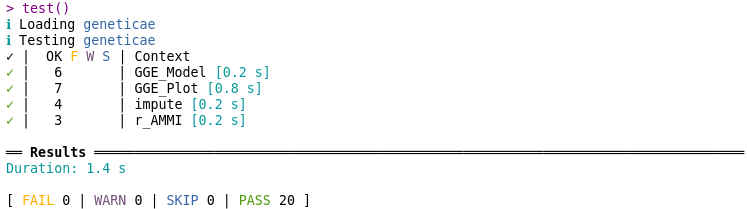
\includegraphics[width=11cm]{./Graficos/Test.png}	
	\end{center}
	\caption{Resultado de correr los tests creados para geneticae}
	\label{fig:fig34}
\end{figure}

Una medida de la calidad de un paquete está dada por el porcentaje de su código que es evaluado durante los testeos. El paquete covr permite hacer ese cálculo, además de mostrar interactivamente qué partes del código fueron evaluadas y cuáles no. Por un lado puede evaluarse en cada archivo .R mediante \textcolor{blue}{devtools::test\_coverage\_file()}, o bien, la cobertura total usando \textcolor{blue}{devtools::test\_coverage()}. El paquete geneticae tiene un porcentaje total de cobertura de los test igual a 16.83\% (Figura \ref{fig:fig35}).


 \begin{figure}[H]
	\begin{center}
		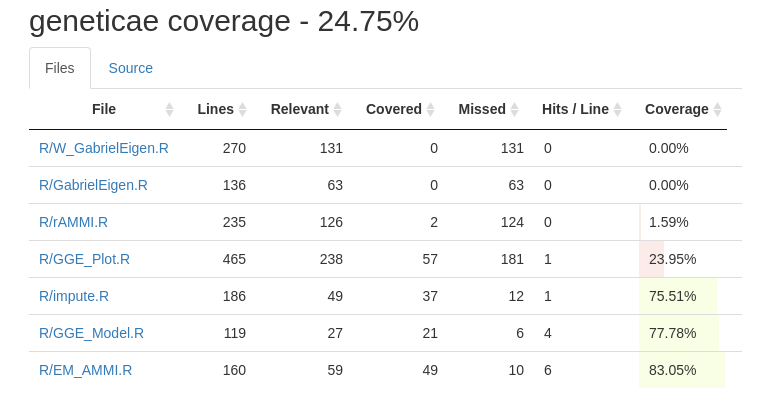
\includegraphics[width=14cm]{./Graficos/Cobertura.png}	
	\end{center}
	\caption{Análisis de cobertura de los tests de geneticae}
	\label{fig:fig35}
\end{figure}

{\LARGE{\textbf{ampliar los test para tener mas cobertura}}}



\subsection{Compilación e instalación}

La función \textcolor{blue}{check}() o R CMD check ejecutado en el shell, es utilizado para verificar que un paquete R esta en pleno funcionamiento. La misma verificará que no haya errores de sintaxis o no se generen warnings. Está compuesto por más de 50 chequeos individuales entre los cuales se encuentran: la estructura del paquete, el archivo descripción, namespace, el código de R, los datos, la documentación, entre otros.  La diferencia con los testeos realizados mediante \textcolor{blue}{use\_testthat}(), es que la última evalúa si las funciones desarrolladan realizan lo deseado, resultando propios de cada paquete. En cambio, lo realizado por R CMD check es común para todos los paquetes. 

Se aconseja realizar verificaciones completas de que todo funciona a medida que se van incorporando funciones ya que si se incorporan muchas y luego se verifican será difícil identificar y resolver los problemas. Una vez que se desarrollaron todos los elementos necesarios para el paquete y no se detectan errores, advertencias o notas, se ejecuta la función \textcolor{blue}{install}(), con el objetivo de instalar el paquete en la biblioteca.


\subsection{Algunos elementos complementarios}

Existen algunas componentes que no son obligatorias a la hora de desarrollar un paquete, pero que ayudan a la comprensión y difusión del mismo.

\subsubsection{Viñetas}

Una viñeta es un tipo especial de documentación que puede agregarse al paquete para dar más detalles y ejemplos sobre el uso del mismo. En ella se brinda es una descripción el problema que el paquete está diseñado para resolver y muestra al lector cómo resolverlo. Se diferencian de las páginas de ayuda en que su adición es opcional y no sigue una estructura fija, dándole la libertad al autor de enseñar de la forma que más le guste cómo usar su paquete.

Muchos de los paquetes existentes tienen viñetas la cuales se pueden encontrar utilizando la función \textcolor{blue}{browseVignettes}(``packagename") si el mismo se encuentra instalado, sino deben consultarse en su página de CRAN, por ejemplo para el paquete \emph{dplyr}: \url{http://cran.r-project.org/web/packages/dplyr}. Cada viñeta proporciona el archivo fuente original, una página HTML o PDF y un archivo de código R. 

Las Viñetas se pueden construir de diversas formas, en este trabajo se utiliza se utiliza \textcolor{blue}{usethis::use\_vignette}(``tutorial\_del\_paquete''). La misma crea un directorio vignettes/, agrega las dependencias necesarias a DESCRIPTION y crea el archivo para redactar la viñeta. 


\subsubsection{Agregar datasets}

A menudo es útil incluir datos en un paquete a fin de proporcionar ejemplos de las funciones incluidas en él. Esto es posible realizarlo con la función \textcolor{blue}{usethis::use\_data}() que crea un archivo .RData y lo almacena en el directorio data/.  Notar que el archivo DESCRIPTION contiene el campo LazyData: true, lo cual genera que los conjuntos de datos no ocupen memoria hasta que sean usados.

Los objetos en la carpeta data siempre se exportan, por lo cual hay que agregar documentación para los mismos. A diferencia de las funciones que son documentadas directamente, para los objetos en data/, se debe crear un archivo y guardarlo en el directorio R/. Esto se puede hacer con roxygen en cualquier Rscript de la carpeta R, aunque se acostumbra juntar toda la documentación para todos los datasets en un único archivo llamado data.R.\\

\subsubsection{Archivo README}

Un archivo README es una forma de documentación de software que contiene información acerca de otros archivos en una carpeta. Usualmente es un archivo de texto plano que permite describir brevemente por qué y para qué alguien tendría que usar el paquete, a la vez que indicar cómo conseguirlo o instalarlo. Se diferencian de la viñeta ya que sólo presenta una descripción breve del paquete.


Para generar el README con R Markdown se utiliza la función \textcolor{blue}{use\_readme\_rmd}() la cual crea un archivo de Rmarkdown con una plantilla donde se escribirá el mismo y será además agregado a .Rbuildignore. Luego, al compilarlo con knitr se obtendrá un archivo README.md, que será la cara visible del paquete si, por ejemplo, en GitHub.

\textbf{badges y logo}

Las insignias o badges son unos íconos que señalan distintas características del paquete, como su nivel de maduración, el nivel de cobertura en el testeo, cantidad de descargas, número de versión, resultado de los controles de CRAN, etc.
Son visualmente muy atractivas y se colocan el en archivo README.     El paquete usethis trae un conjunto de funciones que generan automáticamente el código a incluir en el README.Rmd para agregar los badges: \textcolor{blue}{use\_badge}(badge\_name, href, src), \textcolor{blue}{use\_cran\_badge}(), \textcolor{blue}{use\_bioc\_badge}(), \textcolor{blue}{use\_lifecycle\_badge}(stage), 
\textcolor{blue}{use\_binder\_badge}(sturlpath = NULL) .


Muchos de los paquetes disponibles disponen de un logo con forma hexagonal, que generalmente termina en forma de sticker: los hexStickers. Estos permiten terminar de darle identidad a tu paquete y hacerlo más vistoso. Para crearlos existe el paquete HexSticker. Una vez creado el logo, le podemos pasar su ubicación a la función use\_logo(), que se encargará de darle el tamaño adecuado, guardarlo en la carpeta man del paquete y producir el código de Markdown para incluirlo en el README. 
La Figura \ref{fig:fig36} presenta un fragmento GitHub del paquete geneticae, donde se muestra parte del contenido del archivo README, badges y logo.

\begin{figure}[H]
	\begin{center}
		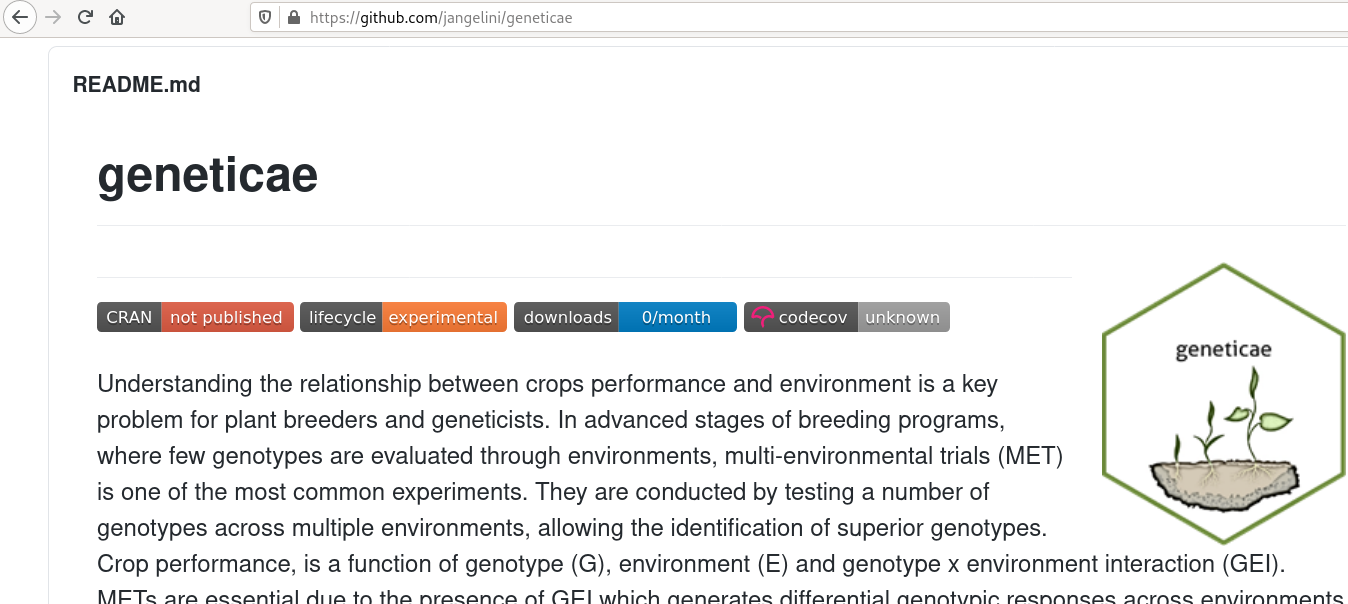
\includegraphics[width=11cm]{./Graficos/badges.png}	
	\end{center}
	\caption{Fragmento de README de geneticae}
	\label{fig:fig36}
\end{figure}




\subsubsection{Archivo NEWS}


Mientras que el README apunta a ser leído por nuevos usuarios, el archivo NEWS es para aquellos que ya usan el paquete.
Este archivo se encarga de contar los cambios presentes en cada versión nueva del paquete que publicamos.
Se sugiere usar Markdown para escribir este archivo y colocar un título principal para cada versión, seguido por títulos secundarios que describen lo realizado (cambios principales, bugs arreglados, etc.).
Si se trata de cambios impulsados por otras personas, por ejemplo, a través de sugerencias hechas en GitHub, se los menciona.
Una buena práctica es ir escribiendo este archivo cada vez que se realiza algo nuevo en el paquete.
La función que nos permite crear este archivo automáticamente es
\textcolor{blue}{usethis::use\_news\_md}(). Hasta el momento, del paquete geneticae solamente se cuenta con la versión de desarrollo (Figura \ref{fig:fig37}) 



\begin{figure}[H]
	\begin{center}
		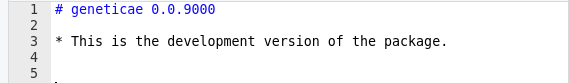
\includegraphics[width=11cm]{./Graficos/News.png}	
	\end{center}
	\caption{Archivo NEWS de geneticae}
	\label{fig:fig37}
\end{figure}





\subsubsection{Crear una página web}

Para mayor visualización del paquete es posible crear una página web \footnote{Para visitar la página web de geneticae debe dirigirse a \url{https://...........}}. El paquete pkgdown está diseñado para la creación de un sitio web de manera rápida y sencilla. Utiliza todo lo creado hasta el momento y lo convierte automáticamente en una pagina web mediante la función \textcolor{blue}{pkgdown::build\_site()}.

 {\LARGE{\textbf{No aparecen los badges en la pag web}}}


\subsubsection{Publicación}


Por último, para que otros usuarios puedan utilizar el paquete es necesario compartirlo en alguno de los repositorios más populares de paquetes de R, entre los cuales se encuentran: CRAN, Bioconductor, GitHub, rOpenSci, R-Forge y RForge. El paquete \emph{geneticae} se encuentra en GitHub, por lo tanto, para instalar el mismo se debe utilizar \textcolor{blue}{devtools::install\_github(``jangelini/geneticae")}.


\section{Shiny APP}
Shiny es un paquete R que permite construir aplicaciones web directamente desde RStudio sin necesidad de conocer en profundidad los lenguajes HTML / CSS / JavaScript . Estas aplicaciones constituyen una interfaz gráfica entre el usuario y R, que permiten realizar un análisis a través de un navegador web sin necesidad de programar.

Una característica importante de las aplicaciones web creadas mediante Shiny es que son dinámicas e interactivas. Para que shiny funcione correctamente, es necesario tener instalado R 3.0.2 o cualquier versión posterior.

\subsection{Estructura de Shiny APP}

Las aplicaciones están compuestas por la interfaz de usuario, ui (\emph{user interfaz}), sección server y la función shinyApp(). 


\textbf{Interfaz del usuario}

La interfaz del usuario (user interface o ui, por sus siglas en inglés) controla el diseño de la aplicación, recibe los inputs y muestra los outputs en el navegador. En general, definir las características de la interfaz puede no resultar tan sencillo ya que muchas de sus herramientas están vinculadas a otros lenguajes de programación, por ejemplo HTML, CSS o JavaScript. Sin embargo, las funciones del paquete shiny facilitan la tarea sin necesidad de conocer en profundidad estos lenguajes.

\textbf{Server}

En la sección server se escribe el código de R que le indica a la app qué debe hacer y cómo debe funcionar, incluyendo la lectura y manipulación de datos, el armado de gráficos, el ajuste de modelos, etc. Para esto, se define una función que debe tener dos argumentos: input y output. Los mismos son listas que almacenan elementos de entrada (datos u opciones elegidas por el usuario a través de la ui) y elementos de salida para mostrar en la app (resultados, tablas, gráficos, mapas, etc.), respectivamente.


\textbf{Ejecución}

Por último, se llama a la función shinyApp(), cuyos dos argumentos principales son ui y server, es decir, cada uno de los elementos definidos anteriormente. Ejecutar esta función da como resultado el lanzamiento de la aplicación, la cual podremos utilizar dentro de RStudio o usando nuestro navegador (Google Chrome, Mozilla Firefox, Microsoft Edge, etc.). Es importante destacar que, al seguir estos pasos, la aplicación sólo funcionará mientras la sesión de RStudio desde la cual se lanzó siga vigente.


\subsection{Desarrollo de Shiny APP}

Una forma de desarrollar una  aplicación es a partir de un nuevo directorio con un sólo archivo llamado app.R, como se muestra a continuación. 

\begin{lstlisting}
library(shiny)
ui<- ...
server<- ...
shinyApp(ui = ui, server = server)
\end{lstlisting}

En este archivo se carga el paquete shiny, se define la interfaz de usuario, la función server y por último, se ejecuta función que permite construir e iniciar una aplicación. Al ejecutar la aplicación la misma aparecerá, de manera predeterminada, en una ventana emergente. Sin embargo, otras dos opciones se pueden configurar desde el menú desplegable de \emph{Run App}. Una de ellas es la ejecución en el panel del visor que permite verla al mismo tiempo que ejecuta el código. La segunda opción es ejecutar en un navegador externo mostrando la aplicación como la mayoría de los usuarios la verán. Dado que la sesión de R estará monitoreando la aplicación y ejecutando las ordenes dadas por el usuario, no se podrá ejecutar ningún comando.

En cualquier lenguaje de programación tener el código duplicado genera un desperdicio computacional y, lo que es más importante, aumenta la dificultad de mantener o depurar el código. Cuando se programa en R, se utilizan dos técnicas para lidiar con el código duplicado: guardar un valor usando una variable o utilizar una función para almacenar un cálculo. Ninguno de estos enfoques son apropiados en una Shiny APP, sino que se utilizan expresiones reactivas. Una expresión reactiva tiene una diferencia importante con una variable: sólo se ejecuta la primera vez que se llama y luego almacena en caché el resultado de la misma hasta que necesite actualizarse. La programación reactiva es un estilo de programación que enfatiza valores que cambian con el tiempo, y cálculos y acciones que dependen de esos valores. Esto es importante para las aplicaciones Shiny porque son interactivas: los usuarios cambian los inputs, lo que hace que la lógica se ejecute en el servidor que finalmente resultan en actualización de los outputs/resultados.

Entre los problemas que pueden surgir al crear una Shiny app se encuentran los errores inesperados, no se obtiene ningún error pero el valor obtenido es incorrecto, o bien todos los resultados son correctos, pero no se actualizan cuando se deben. Una vez localizada la fuente del error, la herramienta más poderosa es el depurador interactivo, éste detiene la ejecución y brinda una consola interactiva donde puede se ejecutar cualquier código para descubrir el error. Para iniciar el mismo, se puede agregar la función browser() en el código fuente, o bien agregar un punto de interrupción RStudio haciendo clic a la izquierda del número de línea.

Al modificar la aplicación, se la ejecuta para poder ver los cambios realizados, por lo tanto resulta esencial reducir la velocidad de iteración. La primera forma acelerar el proceso consiste en escribir el código, utilizar el atajo del teclado Cmd/Ctrl+ Shift+ Enter en lugar del botón ``Ejecutar aplicación'', experimentar interactivamente con la aplicación y cerrar la aplicación, repitiendo este proceso al realizar cualquier cambio. Otra forma de reducir aún más la velocidad de iteración es activar la recarga automática (options(shiny.autoreload = TRUE)) y luego ejecutar la aplicación en un trabajo en segundo plano. Con este flujo de trabajo cuando se guarde un archivo, su aplicación se reiniciará: no es necesario cerrarla y reiniciarla, lo cual conduce a un flujo de trabajo aún más rápido. La principal desventaja de esta técnica es que debido a que la aplicación se ejecuta en un proceso separado, es considerablemente más difícil de depurar.


\subsection{Compartiendo una Shiny Web App}

Una vez creada la aplicación se la publica para su libre uso. En este caso la Shiny Web App encuentra disponible en el servidor de CONICET \url{www.cefobi.com}. Además el proyecto se encuentra en GitHub \url{https://github.com/jangelini/shinyAPP_geneticae}. 
